\documentclass{article}
\usepackage{siunitx}
\usepackage{setspace}
\usepackage{gensymb}                                \usepackage{xcolor}
\usepackage{caption}
%\usepackage{subcaption}
%\doublespacing                                    
\singlespacing                                      \usepackage[none]{hyphenat} 
\usepackage{amssymb}
%\usepackage{relsize}
\usepackage[cmex10]{amsmath} 
\usepackage{mathtools} 
\usepackage{amsmath} 
\usepackage{commath} 
%\usepackage{amsthm}   
%\interdisplaylinepenalty=2500
%\savesymbol{iint}
%\usepackage{txfonts}   
%\restoresymbol{TXF}{iint}  
%\usepackage{wasysym} 
\usepackage{amsthm} 
\usepackage{mathrsfs} 
\usepackage{txfonts}
\let\vec\mathbf{}
%\usepackage{stfloats}
\usepackage{float}
\usepackage{cite}
\usepackage{cases}
\usepackage{subfig}
%\usepackage{xtab}
\usepackage{longtable}
\usepackage{multirow}
%\usepackage{algorithm}
\usepackage{amssymb}
%\usepackage{algpseudocode}
\usepackage{enumitem}
\usepackage{mathtools}
%\usepackage{eenrc}
%\usepackage[framemethod=tikz]{mdframed}
\usepackage{listings}
\usepackage{listings}                              
\usepackage[latin1]{inputenc}                     
%%\usepackage{color}{   
%%\usepackage{lscape}
\usepackage{titling}
\usepackage{hyperref}
%\usepackage{fulbigskip}   
\usepackage{tikz} 
\usepackage{graphicx}
\graphicspath{./sdcard/latex/}
\lstset{		
		frame=single'
	breaklines=true
	}
\newcommand{\mydet}[1]{\ensuremath{\begin{vmatrix}#1\end{vmatrix}}}
\providecommand{\brak}[1]{\ensuremath{\left(#1\right)}}
\providecommand{\norm}[1]{\left\lVert#1\right\rVert}
\newcommand{\solution}{\noindent \textbf{Solution: }}
\newcommand{\myvec}[1]{\ensuremath{\begin{pmatrix}#1\end{pmatrix}}}
\let\vec\mathbf

\begin{document}
\begin{center}
\textbf\large{CHAPTER-9  \\ AREAS OF PARALLELOGRAMS AND TRIANGLES}
\section*{EXCERSISE - 9.2}
\end{center}
\begin{enumerate}
\item $ABCD$ is a parallelogram and $\vec{X}$ is the mid-point of $AB$. If $ ar(AXCD)= 24 cm^2 $ ,then $ar(ABC) =  24 cm^2 $.
\item $PQRS$ is a rectangle inscribed in a quadrant of radius $13 cm$. $\vec{A}$ is any point on $PQ$. If $PS=5 cm$, then $ar(PAS)= 30 cm^2 $
\item $PQRS$ is a parallelogram whose area is $ 180 cm^2 $ and $\vec{A}$ is any point on the diagonal $QS$. The area of $\triangle ASR =90 cm^2$.
\item $ABC$ and $BDE$ are two equilateral triangles such that $\vec{D}$ is the mid-point of $BC$. Then $ar(BDE)=\frac{1}{4}  ar(ABC)$.
\item In Fig.\ref{figs:9.8.}, $ABCD$ and $EFGD$ are two parallelograms and $\vec{G}$ is the mid-point of $CD$. Then$ ar(DPC)=\frac{1}{2}  ar(EFGD)$.
\begin{figure}[h]
	\centering
	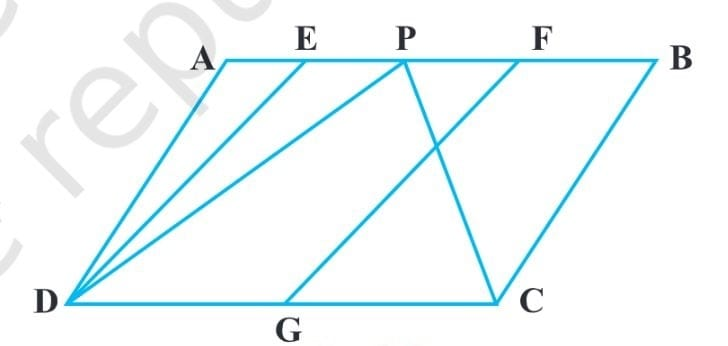
\includegraphics[width=\columnwidth]{figs/9.8.jpg}
	\caption{}
	\label{figs:9.8.}
\end{figure}

\end{enumerate}
\end{document}
